\documentclass{beamer}
\usepackage[utf8]{inputenc}
\usepackage{hyperref}
\usepackage{forloop}
\usepackage{amsmath,amsfonts,amssymb}
\useoutertheme {smoothbars}

\usepackage{listings}
\usepackage{color}
\definecolor{name}{rgb}{0.5,0.5,0.5}
\definecolor{javared}{rgb}{0.6,0,0} % for strings
\definecolor{javagreen}{rgb}{0.25,0.5,0.35} % comments
\definecolor{javapurple}{rgb}{0.5,0,0.35} % keywords
\definecolor{javadocblue}{rgb}{0.25,0.35,0.75} % javadoc

\lstset{language=Java,
	basicstyle=\ttfamily,
	keywordstyle=\color{javapurple}\bfseries,
	stringstyle=\color{javared},
	commentstyle=\color{javagreen},
	morecomment=[s][\color{javadocblue}]{/**}{*/},
	numbers=left,
	numberstyle=\tiny\color{black},
	stepnumber=2,
	numbersep=10pt,
	tabsize=4,
	showspaces=false,
	showstringspaces=false}

\defbeamertemplate*{footline}{smoothbars theme}
{%
	\begin{beamercolorbox}[colsep=1.5pt]{upper separation line foot}
	\end{beamercolorbox}
	\begin{beamercolorbox}[ht=2.5ex,dp=1.125ex,%
		leftskip=.3cm,rightskip=.3cm plus1fil]{title in head/foot}%
		\leavevmode{\usebeamerfont{title in head/foot}\insertshorttitle}%
		\hfill%
		{\usebeamerfont{author in head/foot}\usebeamercolor[fg]{author in head/foot}\insertshortauthor}%
	\end{beamercolorbox}%
	\begin{beamercolorbox}[colsep=1.5pt]{lower separation line foot}
	\end{beamercolorbox}
}

\begin{document}

\title{RESTaurant for Android: Programmierung einer Sitzplatzreservierung \\ Teil III}   
\author{Janis Streib \\ CC-BY-SA} 
\date{02.-06.11.2015} 

\frame{\titlepage} 

\frame{\frametitle{Inhalt}\tableofcontents} 

%\lstinputlisting{filename.java}
%\begin{lstlisting}
% Add code here
%\end{lstlisting}

\section{Android UI}
\subsection{UI}
\frame{\frametitle{Das Android UI}
	\begin{columns}
		\begin{column}{.49\textwidth}
			\begin{enumerate}
				\item Actionbar
				\item Optionmenu
				\item Statusbar
				\item Toast
			\end{enumerate}
		\end{column}
		
		\begin{column}{.49\textwidth}
		%	\begin{picture}(2,2)
		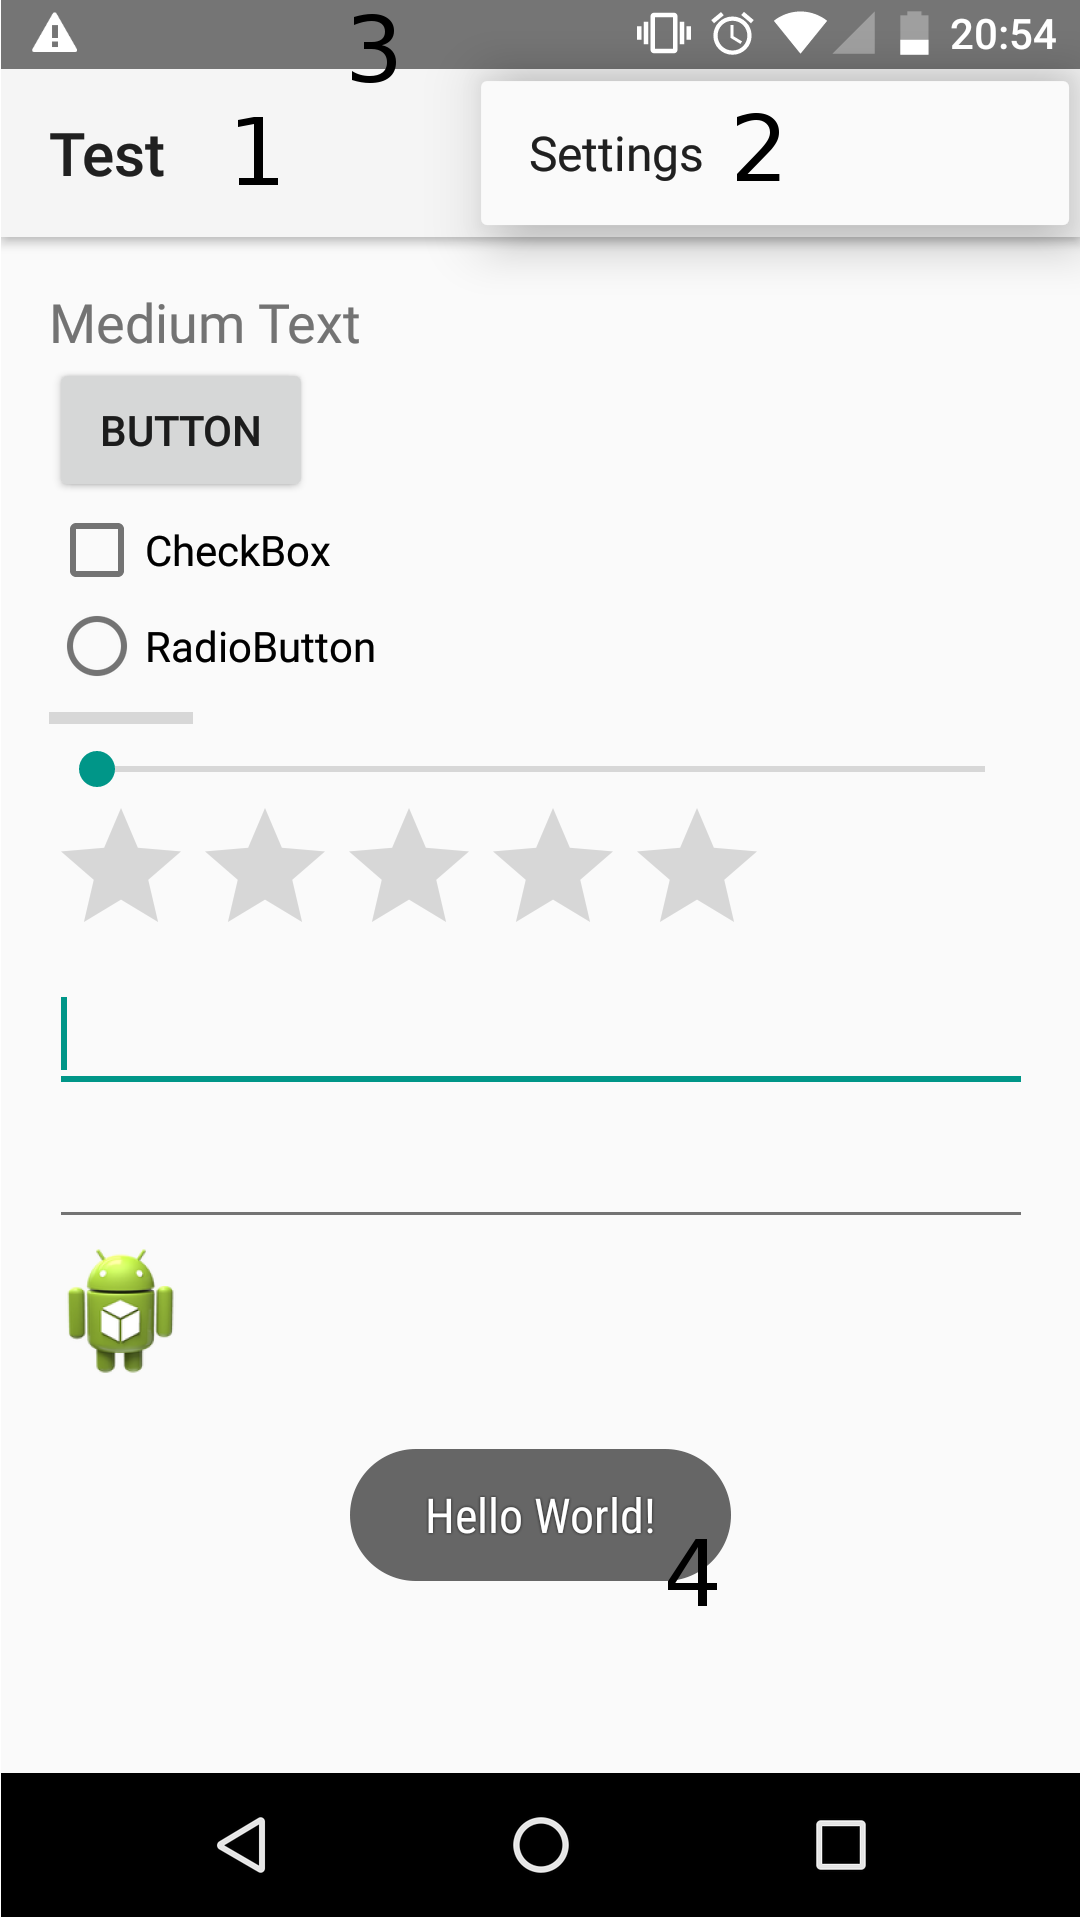
\includegraphics[width=36mm]{img/ui}
		%	\end{picture}
			%\includegraphics[\textwidth]{fig}
		\end{column}
	\end{columns}
	


}
\section{UI-Gestaltung in Android Studio}
\section{UI -> Code}
\section{Ein erster Taschenrechner}
\section{Zustandshaltung}
%\section{Teil IV: Android UI-Design}
%\section{Teil V: Das RESTAurant}
%\section{Optional: Teil VI: Android Design Guidelines}
%\section{Optional: Teil VII: Versionskontrolle}
\end{document}

